% Alur data dan database (lampiran): sekarang Google Sheets, rencana InfluxDB/PostgreSQL di server.
\documentclass[border=4pt]{standalone}
% Gaya bersama gambar deck Demo Day (dipakai semua gambar/*.tex standalone).
\usepackage{amssymb}
\usepackage{fontspec}
\setmainfont{DejaVu Sans Condensed}
\setsansfont{DejaVu Sans Condensed}
\newfontfamily\judulfont{DejaVu Sans}[BoldFont={DejaVu Sans Bold}, Ligatures=TeX]
\usepackage{tikz,pgfplots}
\pgfplotsset{compat=1.18, every axis/.append style={/pgf/number format/assume math mode=true, /pgf/number format/use comma, /pgf/number format/1000 sep={.}}}
\usetikzlibrary{positioning,arrows.meta,calc,shapes.geometric,fit,backgrounds}
\definecolor{gelap}{HTML}{15242B}
\definecolor{teal}{HTML}{285052}
\definecolor{amber}{HTML}{E8A317}
\definecolor{muda}{HTML}{DCE8E8}
\definecolor{abu}{HTML}{8A9499}
\definecolor{teks}{HTML}{1E2B30}
\definecolor{hijau}{HTML}{2F7D5B}
\definecolor{merah}{HTML}{A33A2A}
\color{teks}
\tikzset{
  ubin/.style={fill=muda, rounded corners=5pt, align=center, inner sep=6pt},
  inti/.style={ubin, fill=gelap, text=white},
  panah/.style={-{Stealth[length=3mm]}, line width=1.3pt, draw=amber},
  panahabu/.style={-{Stealth[length=2.5mm]}, line width=1pt, draw=abu},
  judulubin/.style={font=\judulfont\bfseries},
}
% Dibuat otomatis oleh buat_aset.py dari ml/results/energi_harian.json; jangan diedit manual.
\newcommand{\energiTurbin}{270}
\newcommand{\energiQa}{187}
\newcommand{\energiQb}{377}
\newcommand{\hariEnergi}{140}
\newcommand{\raspiWh}{71}
\newcommand{\chipWh}{4,1}
\newcommand{\raspiPersen}{26}
\newcommand{\chipPersen}{1,5}
\newcommand{\raspiPersenA}{19}
\newcommand{\raspiPersenB}{38}
\newcommand{\raspiPersenNum}{26.3}
\newcommand{\chipPersenNum}{1.5}
\newcommand{\hematKwh}{24}
\newcommand{\kaliHemat}{17}
\newcommand{\jRaspi}{182}
\newcommand{\jChip}{10,4}
\newcommand{\periodeEnergi}{2026-03-31--2026-10-20}

\AtBeginDocument{\hyphenpenalty=10000 \exhyphenpenalty=10000}

\begin{document}
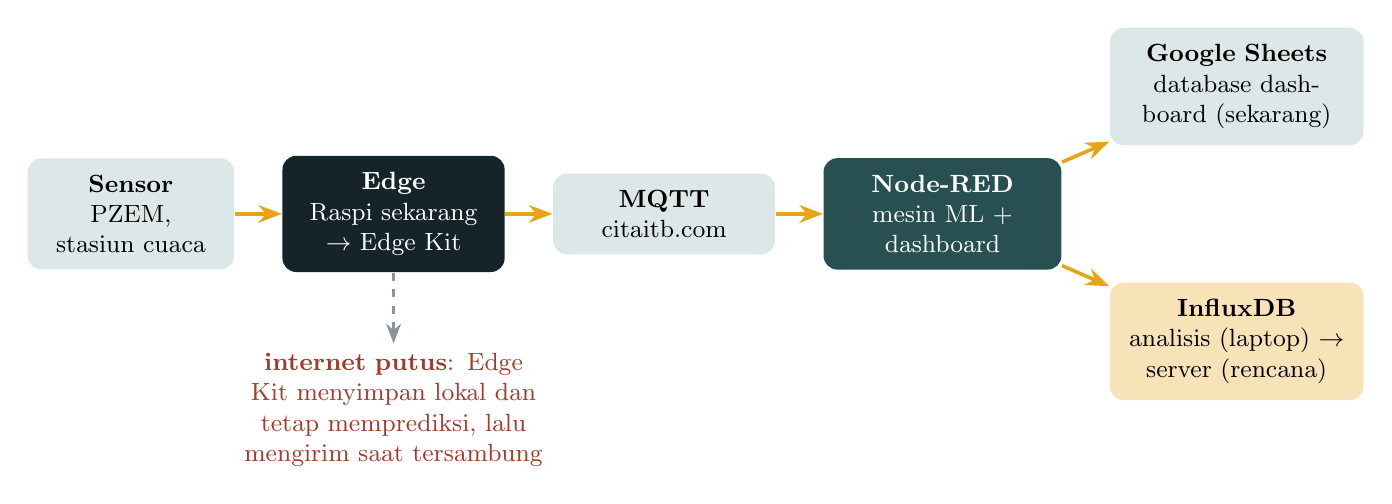
\begin{tikzpicture}[font=\fontsize{9}{11}\selectfont, node distance=0.55cm and 0.6cm]
  \node[ubin, text width=2.2cm] (s) {\textbf{Sensor}\\PZEM, stasiun cuaca};
  \node[inti, text width=2.4cm, right=of s] (e) {\textbf{Edge}\\Raspi sekarang\\$\to$ Edge Kit};
  \node[ubin, text width=2.4cm, right=of e] (m) {\textbf{MQTT}\\citaitb.com};
  \node[inti, fill=teal, text width=2.6cm, right=of m] (n) {\textbf{Node-RED}\\mesin ML + dashboard};
  \node[ubin, text width=2.8cm, above right=0.15cm and 0.6cm of n] (g) {\textbf{Google Sheets}\\database dashboard (sekarang)};
  \node[ubin, fill=amber!30, text width=2.8cm, below right=0.15cm and 0.6cm of n] (i) {\textbf{InfluxDB}\\analisis (laptop) $\to$ server (rencana)};
  \draw[panah] (s) -- (e); \draw[panah] (e) -- (m); \draw[panah] (m) -- (n);
  \draw[panah] (n) -- (g); \draw[panah] (n) -- (i);
  \node[below=0.9cm of e, text width=4.2cm, align=center, text=merah] (b) {\textbf{internet putus}: Edge Kit menyimpan lokal dan tetap memprediksi, lalu mengirim saat tersambung};
  \draw[panahabu, dashed] (e) -- (b);
\end{tikzpicture}
\end{document}
